
\section{Usage}\label{sec:usage}

To install Pecan see the instructions at \url{https://github.com/ReedOei/Pecan}.

\subsection{Running Pecan}

The standard method of using Pecan is to create a new file (with a \texttt{.pn} extension) which will hold all definitions and theorems.
Then the file can be run using the following command on most operating systems (whether you use \texttt{python3} or \texttt{python} depends on how Python is installed):

\begin{lstlisting}[language=bash, basicstyle=\normalsize\ttfamily]
$ python3 pecan.py FILENAME
\end{lstlisting}

You can also run the file in \textbf{interactive mode}, which will run the file and then allow you to directly type new definitions and directives with the definitions from the file loaded:

\begin{lstlisting}[language=bash, basicstyle=\normalsize\ttfamily]
$ python3 pecan.py -i [FILENAME]
\end{lstlisting}

\subsection{A First Theorem}

For a taste of Pecan's syntax and the sort of theorems we can prove using Pecan, we'll prove a simple theorem about natural numbers:

\begin{theorem}
Every natural number is either even or odd.
\end{theorem}

Pecan has a built-in definition of natural numbers, which we will use to write a definition of ``even'' for natural numbers \footnote{Pecan also has an \texttt{even} predicate in its standard library, called \texttt{even}, however, we will write our own for instruction purposes.}.
The primary method of defining predicates in Pecan is the following:

\begin{pecan}
PREDICATE_NAME(ARGUMENTS) := BODY
\end{pecan}

In our particular case, we can define a number to be even if there is another number that is half of it.
We write this definition in Pecan as:

\begin{pecan}
is_even(x is nat) := existsy is nat. x = 2*y
\end{pecan}

Let's unpack this definition a little.
First, we say that \pecaninline{x is nat} in the arguments of \pecaninline{is_even} so that Pecan knows the \textbf{type} of the arguments, and we do the same on the existential quantifier for \pecaninline{y}.
Specifying the type allows Pecan to lookup the appropriate arithmetic operator definitions (e.g., for addition).
You can think of \pecaninline{x is nat} as being equivalent to $x \in \N$.
The body of the predicate, \pecaninline{existsy is nat. x = 2*y} works almost exactly like in a standard mathematical definition; \pecaninline{is_even(x)} is true if and only if \pecaninline{existsy is nat. x = 2*y}.

Note that instead of writing \pecaninline{x is nat} all the time, we can \textbf{restrict} certain variables to only be a specific type using the \pecaninline{Restrict} directive.
Let's do that for a few variables:

\begin{pecan}
Restrict x,y,z are nat.
\end{pecan}

Note that above \pecaninline{are} is just another way to write \pecaninline{is}.
We can get an example of a number that this predicate accepts with the following line.

\begin{pecan}
Example using natFormat of { is_even(x) }.
\end{pecan}

\begin{pecan_output}
[(x,0)]
\end{pecan_output}

That is, one input that \pecaninline{is_even} accepts is $0$, which makes sense, because $0$ is a natural number and $0$ is even.
Natural numbers in Pecan are, by default, in LSD (least-significant digit first) format, which is the reverse of the standard order; this order makes the underlying implementation significantly easier.
We can ask Pecan for more interesting examples as well.
For example, we can ask for an odd number greater than 33 by writing the following:

\begin{pecan}
is_odd(x) := existsy. x = 2*y+1
Example using natFormat of { x > 33 & is_odd(x) }.
\end{pecan}

We omitted the \pecaninline{x is nat} and \pecaninline{y is nat}; this omission is allowed because of the restriction we placed on \pecaninline{x} and \pecaninline{y}.
When we run the file, Pecan responds with:

\begin{pecan_output}
[(x,49)]
\end{pecan_output}

Again, this answer makes sense: it is an odd number, and it is greater than 33.
This particular feature is non-deterministic---you may not get the same examples inputs that we show here.
Also note that this output has been pretty-printed---if you want the raw input string, which will be an infinite binary string, you can instead use:

\begin{pecan}
Example using stdFormat of { x > 33 & is_odd(x) }.
\end{pecan}

This command gives me \pecaninline{[(x,100011(0)^w)]}, meaning that the input string starts with \pecaninline{100011} and then is \pecaninline{0} repeated infinitely many times.

Now that we've explored Pecan a little bit, let's write the actual theorem, and ask Pecan to check it.

\begin{pecan}
Theorem ("All natural numbers are even or odd", {
    forallx. is_even(x) | is_odd(x)
}).
\end{pecan}

Pecan proves the theorem is true, which the following output indicates.

\begin{pecan_output}
[INFO] Checking if All natural numbers are even or odd is true.
$\text{\color{ForestGreen}All natural numbers are even or odd is true.}$
\end{pecan_output}

We can see this theorem is true in another way, by confirming that a natural number is odd if and only if it is not even.

\begin{pecan}
Theorem ("x is odd if and only if it is not even", {
    forallx. is_odd(x) <=> !is_even(x)
}).
\end{pecan}

Again, Pecan confirms this theorem:

\begin{pecan_output}
[INFO] Checking if x is odd if and only if it is not even is true.
$\text{\color{ForestGreen}x is odd if and only if it is not even is true.}$
\end{pecan_output}

Below are some more involved examples with somewhat less in-depth explanation.
Note that Pecan allows the use of Unicode characters such as $\exists$, and $\forall$, which we tend to use for readability, but it also supports using the words $\color{blue} \texttt{exists}$ and $\color{blue} \texttt{forall}$.

\subsection{Examples}

\subsubsection{Example: The Chicken McNugget Problem }

Henri Picciotto asked the following problem in his algebra textbook \cite{picciotto1994algebra}:

\begin{quote}
    What is the greatest number of chicken nuggets that cannot be ordered using only boxes of 6, 9, and 20?
\end{quote}

We call all such numbers that can be ordered \term{purchasable}, and we can define them in Pecan as follows:

\begin{pecan}
Restrict n,m,a,b,c $\color{red} \in$ binary.
purchasable(n) := existsa,b,c. n = 6*a + 9*b + 20*c
\end{pecan}

We can then define the largest non-purchasable number in the natural way to be:
\begin{pecan}
largest(n) := !purchasable(n) & forallm. if !purchasable(m) then m <= n
\end{pecan}

Pecan produces the automaton in Figure~\ref{fig:largest_non_purchasable} for us, which tells us that the largest non-purchasable number is $101011_2$, or $43$ in base 10.

\begin{figure}
    \centering
    \includegraphics[width=\textwidth]{images/largest_not_purchasable.pdf}
    \caption{A B\"uchi automaton accepting $110101$ in least significant digit first representation.}
    \label{fig:largest_non_purchasable}
\end{figure}

Note that we can also simply ask Pecan to tell us the number, by writing
\begin{pecan}
Example using natFormat of { largest(n) }.
\end{pecan}
which gives us
\begin{pecan_output}
[(n,43)]
\end{pecan_output}

We can simplify our code using Pecan's built-in \pecaninline{max} keyword (there are similar keyworsd for \pecaninline{min}, \pecaninline{inf}, and \pecaninline{sup}):
\begin{pecan}
largest(n) := n = max { m : !purchasable(m) }
\end{pecan}

\subsubsection*{Example: Properties of the Thue-Morse Word}

Below, we develop a Pecan program that proves two well-known properties of the Thue-Morse word, $T$, which is defined by: the $n$-th digit of the Thue-Morse word, $T[n]$, is $1$ if the binary representation of $n$ has an odd number of $1$'s, and $0$ otherwise \cite{auto_seq}.

The Thue-Morse word starts with: $1101001100101101001011001101001\ldots$
\begin{definition}
    A word $w$ is a \textbf{square} if it is of the form $w = xx$ for some nonempty word $x$.
    Similarly, $w$ is a \textbf{cube} if it is of the form $w = xxx$ for some nonempty word $x$.
\end{definition}

\begin{theorem}\cite{auto_seq}
    The Thue-Morse word contains squares, but does not contain any cubes.
\end{theorem}

Here is the equivalent definition of $T$ in Pecan (\texttt{odd\_ones} is defined as an automaton):
\begin{pecan}
T(x) := odd_ones(x)
\end{pecan}

Below are definitions of square and cube for the Thue-Morse word in Pecan.

\begin{pecan}
Restrict i,j,n $\color{red} \in$ binary.
square(i, n) := n > 0 $\color{red} \wedge$ T[i $\color{red} \ldots$ i+n] =$\ $T[i+n $\color{red} \ldots$ i+2*n]
cube(i, n) := square(i, n) $\color{red} \wedge$ square(i+n, n)
\end{pecan}


Finally, we state the theorems we would like to prove, and ask Pecan to attempt to prove that there are squares, but there are no cubes.

\begin{pecan}
squares_exist() := $\exists$i. $\exists$n. square(i, n)
#assert_prop(true, squares_exist)
cubes_exist() := $\exists$i. $\exists$n. cube(i, n)
#assert_prop(false, cubes_exist)
\end{pecan}

The output from Pecan is the following, indicating that the theorem is true.
\begin{pecan_output}
[INFO] Checking if squares_exist is true.
$\text{\color{ForestGreen}squares\_exist is true.}$
[INFO] Checking if cubes_exist is false.
$\text{\color{ForestGreen}cubes\_exist is false.}$
\end{pecan_output}

Here is another theorem about the Thue-Morse word that we can check.
\begin{theorem}\cite{zbMATH01737190}
There are no overlapping squares, i.e. words of form $0x0x0$ or $1x1x1$ for some nonempty word $x$. 
\end{theorem}

We can express this theorem in Pecan as:

\begin{pecan}
o_square(i, n) := n > 0 & square(i,n) & T[i] = T[i+2*n]
o_squares_exist() := existsi,n. o_square(i, n)
#assert_prop(false, o_squares_exist)
\end{pecan}

Pecan verifies the theorem: 

\begin{pecan_output}
[INFO] Checking if o_squares_exist is false.
$\text{\color{ForestGreen} o\_squares\_exist is false.}$
\end{pecan_output}

\begin{definition}
    A rational number $e$ is an \term{exponent} of a finite word $w$ if $e = |w| / p$ where $p$ is a period of $w$.
\end{definition}

\begin{definition}
    The \term{critical exponent} of a word $w$ is the supremum of all exponents of subwords of $w$.
\end{definition}

\begin{theorem}
    The critical exponent of the Thue-Morse word is $2$.
\end{theorem}
\begin{proof}
As proven by Pecan, there are squares in the Thue-Morse word, so it is possible to achieve an exponent of $2$.
However, there are no overlapping squares, which means we cannot have an exponent greater than $2$---a subword with an exponent greater than $2$ will have more than $2$ periods, which would be an overlapping square.
\end{proof}

This example demonstrates a common use case of theorem provers like Pecan: we can automate the tedious parts of a proof, allowing us to prove the theorem from a ``high-level'' perspective.

Next, we'll prove that the Thue-Morse word has a factor with least period $p$ for every $p > 0$, recovering a result of \autocite[Theorem 2]{Currie2009LeastPO}.
To do so, we begin by defining periods in Pecan:
\begin{pecan}
Restrict i,j,k,n,p,r is binary.
p is period(i,j) :=
    p > 0 & i is binary & j is binary & p is binary &
    forallk. if i <= k & k < j - p then T[k] = T[k+p]
\end{pecan}

Now we can simply state the theorem:
\begin{pecan}
Theorem ("For every p > 0, the Thue-Morse word has a factor with least period p.", {
    forallp. if p > 0 then existsi,j. p = min { n : n is period(i,j) }
}).
\end{pecan}

\reed{This stuff might be a little complciated for a ``tutorial'', but basically I found this paper~\cite{Currie2009LeastPO} and it turns out we can reprove a lot of the results they prove for the Thue-Morse word automatically, which is interesting. Not sure where it should go though.}

\reed{This theorem is a corollary of Lemma 3 of~\cite{Currie2009LeastPO} (at least, that's what they claim), which we can automatically prove}
\begin{theorem}
    The Thue-Morse word contains an unbordered factor of length $r$ for every $r \not\equiv 1 \pmod{6}$.
\end{theorem}
\begin{proof}
Using Pecan, the proof is straightforward.
We define an unbordered factor as a factor $w$ whose least period is $|w|$, and then use Pecan to directly state and prove the theorem:
\begin{pecan}
unbordered(i,n) := n = min { p : p is period(i,i + n) }
Theorem ("The Thue-Morse word has an unbordered factor of length r when r != 1 (mod 6).", {
    forallr. if r > 0 & !(existsk. r = 6*k + 1) then existsi. unbordered(i,r)
}).
\end{pecan}
\end{proof}

We are also able to answer the following question, which they claim is open \reed{although that was in 2009, regardless, it's nice we can automatically answer their question (if this counts as an answer)...}.

\reed{UPDATE: Jeffery shallit told me on reddit that he already used walnut to solve this problem (\url{https://link.springer.com/chapter/10.1007/978-3-642-37064-9_27}). Still a good example, I think.}

\reed{actually it was a slightly different question that they claim is open which we can also answer but I just haven't written yet.}

\begin{theorem}
    If $r \equiv 1 \pmod{6}$, then the Thue-Morse contains an unbordered factor of length $r$ when $r$ is of the form $1|10^*1(01^*0)^*10^*(1(01^*0)^*1)^*11$.
    % A more standard programming-language compatible regex is: 1+10*1(01*0)*10*(1(01*0)*1)*11
\end{theorem}
\begin{proof}
We create the automaton in Figure~\ref{fig:unbordered_1_mod_6} using the following Pecan code.
Note that we use the \term{annotation} \pecaninline{@postprocess}, which tells Pecan to try to simplify the automaton representing a property.
It is not necessary, but it makes it easier to inspect the resulting automaton.
\begin{pecan}
unbordered_1_mod_6(n) := @postprocess[
    existsi. (existsk. n = 6*k + 1) & unbordered(i,n)
]
#save_aut("unbordered_1_mod_6.aut", unbordered_1_mod_6)
\end{pecan}

Then the theorem is proved by manual inspection of the automaton.

\begin{figure}
    \centering
    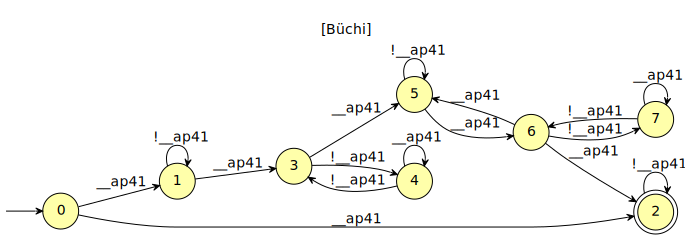
\includegraphics[width=0.7\textwidth]{images/unbordered_1_mod_6.pdf}
    \caption{A B\"uchi automaton accepting $(1|10^*1(01^*0)^*1(0^*(1(01^*0)^*1)^*11)0^{\omega}$ in least significant digit first representation.}
    \label{fig:unbordered_1_mod_6}
\end{figure}

\end{proof}
